\documentclass[authordate, meta, issue]{jote-new-article}

\usepackage{caption}

\usepackage{tabularx}

\usepackage{graphicx}

\usepackage{hyperref}

\usepackage[backend=biber,style=apa]{biblatex}


\PassOptionsToPackage{absolute,overlay}{textpos}
\RequirePackage{xcolor}
\usepackage{tikz}

\addbibresource{bibliography.bib}

\jotetitle{Issues in clinical studies leading to medical research ethics committee (MREC) negative decisions}
\keywordsabstract{clinical trials, clinical studies, research assessment, medical research ethics committee, medical research ethics}
\abstracttext{The rationale behind a Medical Research Ethics Committee (MREC) negative decision is always shared directly with the applicants. However, insight into the review process and common reasons for a negative decision may also be valuable for other researchers, clinical research organizations and people with an interest in MREC processes. To our knowledge Medical Research Ethics Committees (MRECs) do generally not report on the negative decisions they issue and on the underlying rationale for such decisions. Here we give insight into the MREC review process by briefly describing procedures and discussing the negative decisions issued by MREC NedMec in the past five years.}
\runningauthor{Heinsbroek et al.}
\jname{Journal of Trial \& Error}
\jyear{2024}
\acknowledgments{We thank Myriam van der Loo, Jan Paul de Boer and Bianca Goemans for commenting on the draft of this paper.
}
\paperdoi{10.36850/21gx-cy60}
\paperreceived{October 12, 2023}
\author[1]{\mbox{Sigrid E. M. Heinsbroek\orcid{0000-0003-0971-8599}}}
\affil[1]{METC NedMec, Utrecht, the Netherlands}
\corremail{\href{mailto:s.e.m.heinsbroek@umcutrecht.nl}{s.e.m.heinsbroek@umcutrecht.nl}}
\corraddress{METC NedMec}
\runningauthor{Heinsbroek et al.}
\author[1]{\mbox{Vincent Bontrop\orcid{0000-0003-4009-0939}}}
\author[1]{\mbox{Rutger P. Chorus}}
\author[1]{\mbox{C. Michel Zwaan\orcid{0000-0001-6892-8268}}}
\paperaccepted{January 11, 2024}
\paperpublished{March 22, 2024}
\paperpublisheddate{2024-03-22}
\jwebsite{https://journal.trialanderror.org}

\setcounter{page}{17}
\jissue{2}
\jvolume{4}
\jpages{17-23}
\specialissue{Scientific Failure and Uncertainty in the Health Domain}
\articletype{Special Issue - Meta-Research}

\begin{document}
\begin{frontmatter}
  \maketitle
  \begin{abstract}
    \printabstracttext
  \end{abstract}
\end{frontmatter}








\lettrine{I}{n} the Netherlands, medical scientific research in which human volunteers are subjected to procedures, or are required to follow rules of behavior, needs to be reviewed by an accredited MREC, as per the Dutch law for "Medical Research involving Human Subjects". The Netherlands has 14 accredited MRECs and their operations are overseen by the Central Committee on Research Involving Human Subjects (CCMO).

\begin{tikzpicture}[remember picture, overlay]
    \node[align=left, text width=15cm, anchor=north west] 
    at ([xshift=4.7cm, yshift=-0.3cm]current page.north west) 
    {
        \noindent{\textbf{Correction notice}} \\
        Incorrect Special Issue Labeling (Article erroneously excluded): This article was previously not labeled as part of a special issue due to an error. This has now been corrected.\vspace{2pt}
        \noindent{{\color{joteorange}\rule{\linewidth}{1pt}}}
    };
\end{tikzpicture}

MRECs determine if studies comply to the current legislation, regulations and guidelines concerning human subject research. This includes the General Data Protection Regulation (GDPR; European Parliament and the Council of the European Union, 2016), the Medical Research Involving Human Subjects Act (WMO; Nederlandse Overheid, 2022), the Clinical Trial Regulation (CTR; European Parliament and the Council of the European Union, 2014) or the Clinical Trial Directive (CTD, till 31\textsuperscript{st} of January 2022; European Parliament and the Council of the European Union, 2001), Medical Device Regulation (MDR; European Parliament and the Council of the European Union, 2021), In Vitro Diagnostics Regulation n (IVDR; European Parliament and the Council of the European Union, 2017), guideline for Good Clinical Practice (European Medicines Agency, 2016), Dutch Embryo Act (Nederlandse Overheid, 2021) and the Declaration of Helsinki (World Medical Association, 2013). The kind of documents needed for assessment, the way a dossier is submitted, and the committee that assesses a research protocol depends on legislation and the regulations applicable to the study. With the increase in regulation, it becomes more common that submitted studies are returned to the applicant because of mistakes in the submission procedures or documents. For instance, clinical trials with medicinal products are sometimes still submitted directly to the MREC, while these should now be submitted via the Clinical Trials Information System (CTIS). Furthermore, medical device studies are not always submitted as an MDR-study, and as a result documents may be missing. Only when the study is submitted correctly and all essential documentation is available, the review process can start.







\section{MREC review process}



In the Dutch review process, medical ethical, regulatory and scientific assessment is integrated leading to a thorough review system which is, to the best of our knowledge, unique in the world. A submitted study will be reviewed in a plenary MREC committee meeting where the presence of the following experts is mandatory:

\begin{itemize}
  \item a medical doctor,



  \item a lawyer,



  \item an ethicist,



  \item a methodologist/statistician,



  \item a patient advocate specifically for the perspective of the human subject.


\end{itemize}

For specific cases, further experts are required to be part of the committee:


\begin{figure}[b!]
  \begin{fullwidth}
    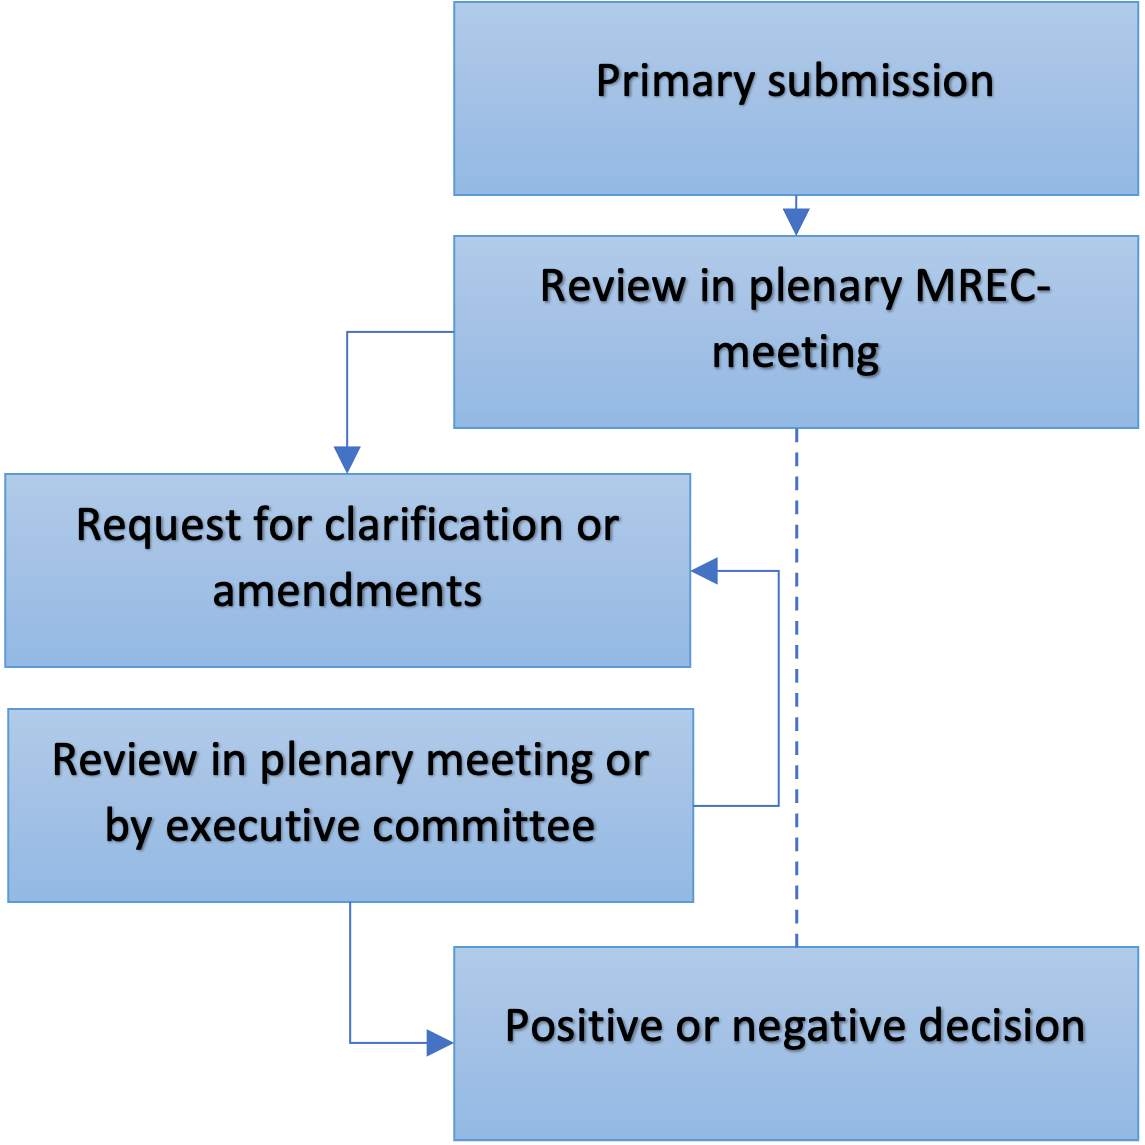
\includegraphics[width=\linewidth]{media/Picture1.png}

    \caption{\emph{Stages of the MREC review process.}}
  \end{fullwidth}
\end{figure}
\begin{itemize}

  \newpage


  \item a pediatrician (obligatory for research conducted with minors),



  \item
        a clinical pharmacologist (for clinical trials with medicinal products),



  \item a hospital pharmacist (for clinical trials with medicinal products),



  \item
        a medical device expert (for clinical investigations with medical devices).


\end{itemize}

Every expert meets strict requirements and is approved by the CCMO before taking part in an MREC (CCMO, 2020). Together the committee assesses the study by weighing benefit versus participant burden and risk. They take into account:


\begin{itemize}


  \item if it is likely that the scientific research will lead to the discovery of new insights in the field of medical science,



  \item
        if there are alternatives to the submitted study available that reduce burden or risk of participants, and



  \item if the interests of the subject or other current or future patients are served by the research.


\end{itemize}

The committee pays close attention to safety and ethical aspects. The latter includes the informed consent procedure in which it is of upmost importance that participants are clearly informed of the purpose and the potential benefit but also the risks of the study. Contracts will be reviewed based on CCMO guidelines on the review of research contracts (CCMO, 2011)  and should not contain unreasonable restrictions regarding the disclosure of the results, or premature termination of the study, or unreasonable financial incentives. Furthermore, it should be clear that the study design enables researchers to answer the research question, that enough study participants can be recruited and included, and that the available funds will cover the costs of the whole study to completion.



The review process of MREC NedMec is depicted in figure 1. After the first review by the committee, questions are sent to the investigators. Depending on the kind of questions asked, the further assessments will either be done in a plenary meeting when the committee requires substantial modifications or will be delegated to an executive committee when only minor issues need to be resolved (fig.1).

























































\begin{figure}[t!]
  \begin{fullwidth}
    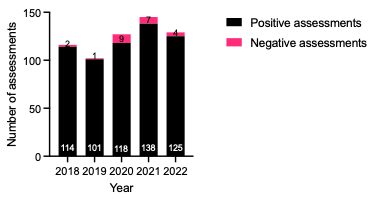
\includegraphics[width=\linewidth]{media/Picture2.png}

    \caption{\emph{Number of primary assessments by METC NedMec over five years (2018 to 2022).}\\
      The number of positive and negative decisions made by METC NedMec over the course of five years.}

    \label{fig:rId12}

  \end{fullwidth}
\end{figure}


\section{Negative decisions}



Negative decisions are relatively uncommon. In the last three years, only 1.7\% of the studies that have been assessed in the Netherlands by an accredited MREC or the CCMO received a negative decision (CCMO, 2023) . A negative decision is rarely given after the first MREC review of the study. Depending on whether the applicable legislation offers the possibility to request additional information and modifications multiple times, generally two or more rounds of discussion take place before a negative decision is issued. Under CTR this is limited to one round of questions.







Over the last five years MREC NedMec (known as METC Utrecht until 2021) assessed 596 studies, of which 23 received a negative decision (fig. 2). The number of negative decisions peaked in 2020, which was most likely due to a large number of COVID-19 studies that were submitted under time pressure (METC Utrecht, 2020).



In the next paragraph we will discuss the reasons that led to negative decisions by MREC NedMec in the last five years (2018 to 2022) regarding studies that are subject to the WMO. These are summarized in Figure 3.







\subsection{Incomplete research file}



In this period most negative decisions were given due to an incomplete research file despite rounds of questions. For instance, when a protocol is submitted as a WMO-study while a medicinal product or a medical device is used, one may forget to submit quality or safety information on the medicinal product or device.







\subsection{Scientific validity or safety}



It occasionally happened that scientific justification remained incomplete, and in most of these studies the lack of sufficient quality or safety information led to a negative decision. For example, it happened that a study was submitted as a phase IB/IIA study, while the requirements for a phase I and II study are different, and information on the data safety monitoring board, safety criteria and post-trial access were missing, and not handled well in the answer to the committee review. When safety information was sufficient, the intervention could be considered too burdensome compared to the scientific contribution, which led to negative decisions in three studies.







\subsection{Benefit/risk assessment}



Surprisingly, in more than 20\% of the negative decisions, researchers could not sufficiently substantiate the burden and risks for the study participant. In these studies, the MREC's questions about necessity of the study were often answered briefly without a balanced benefit/risk assessment. For example, under Dutch law it is forbidden to conduct scientific research with children under 16 years of age unless these children perceive some benefit from the study, or when the study cannot be carried out without their cooperation (Nederlandse Overheid, 2022). Two studies received a negative decision because the added scientific value for including children remained unclear. For one study the committee was convinced of its relevance, but insurance for the children to cover any potential damage incurred as a result of participating in the study could not be arranged. This also resulted in a negative decision.







\subsection{Consent procedure and study design}



Despite rules and guidelines on how informed consent should be obtained (CCMO), two studies received a negative decision due to an unacceptable procedure to obtain informed consent. In one study researchers deemed it unnecessary to ask for consent, which the committee did not agree with. In the other study researchers intended to directly phone potential study participants for research purposes, without knowing if they were willing to participate. Some studies received a negative decision based on improper study design. For example, results could not be directly attributed to the intervention because of a missing control group, or a subjective primary endpoint was used which was more likely to give an unreliable answer to the study question.



\begin{figure*}
  \begin{fullwidth}
    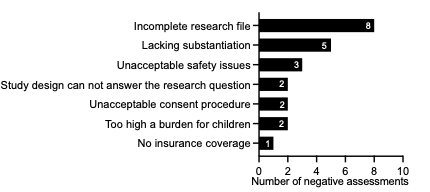
\includegraphics[width=\linewidth]{media/Picture3.png}

    \caption{\emph{Reasons for negative decisions by MREC NedMec over five years (2018 to 2022).}}

    \label{fig:rId13}

  \end{fullwidth}
\end{figure*}


\subsection{Appeal}



After receiving a negative decision most studies were modified and resubmitted for a new review, but there is also the possibility to appeal the MREC decision at the CCMO. Less than half of the negative decisions were appealed (fig 4). Of the six studies that were appealed, two had received a negative decision due to the consent procedure, one due to the burden for children, one due to safety issues, and one due to missing substantiation of the risk-benefit assessment. Three appeals were withdrawn after discussion with the CCMO. Three other appeals received an unfounded verdict by the CCMO after appeal, meaning that the MREC decision remained valid and unchanged. In the one study where the appeal was founded, researchers submitted new information which affected the risk-benefit assessment and helped in the final decision. This might also have led to a positive decision by METC NedMec, if the information was available at the time of review. Together this shows that while appeal is an option, investigators may be better off by adjusting the study or providing the information asked for by the MREC.



\begin{figure}
  \begin{fullwidth}

    
\includegraphics[width=\linewidth]{media/Picture4.png}

    \caption{\emph{Appeal at the Central Committee on Research Involving Human Subjects (CCMO)}\\
      Number of studies that received a negative decision by METC NedMec between 2018 and 2022. The majority of decisions were not appealed. When the decision was appealed there were three possible outcomes: 1) appeal founded, 2) appeal unfounded, 3) appeal was withdrawn after a first conversation with the CCMO.}

    \label{fig:rId14}
  \end{fullwidth}
\end{figure}







\section{Recent changes in regulation and their consequences}



Until the introduction of the ECTR, the role of the competent authorities in the Netherlands was limited, and the assessment was done in a decentralized fashion by the accredited MRECs. These would assess the entire dossier (now referred to as part I and part II under the ECTR). Currently, studies subject to the CTR or certain articles of the MDR and IVDR will have a validation period in which completion of the study file is checked and missing information is requested. This should prevent negative decisions caused by submitting an incomplete dossier. However, since the CTR came into effect on January 31, 2022, it seems that the number of negative decisions for clinical trials with medicinal products may be increasing. In the last year, METC NedMec issued three negative decisions out of 31 studies assessed under CTR (9,6\%). In the year before, two out 55 clinical trials with medicinal products assessed under CTD received at negative decision (3,6\%). In our opinion, the following factors contribute to a higher number of negative decisions:

\begin{itemize}


  \item Researchers are still unfamiliar with the CTR and the different available guidelines, resulting in research files that do not meet the requirements that apply under the CTR.



  \item
        Deadlines are tighter, and the 12 days to comply is often too short for investigators to make major changes when information or whole documents are missing.



  \item Studies subjected to the CTR only have one round of review, after which a decision needs to be made.



  \item
        Particularly in assessments of international studies, where one country is appointed as the reporting member state, it happens that questions deemed essential by a concerned member state are removed in the communication to investigators. This leads to negative decisions on conducting the study in The Netherlands.


\end{itemize}
\newpage
Together these changes will most likely increase the number of MREC negative decisions further in the future. Furthermore, appeal against a negative decision under CTR at the CCMO is not always possible; in that case the study needs to be resubmitted.







\section{Conclusion}

Medical ethical and scientific review is strongly integrated in the Dutch MREC process leading to a thorough assessment. Negative decisions are uncommon, and researchers can support quick and positive MREC review by submitting complete and well-substantiated studies in the correct manner, according to the regulations applicable to the study. It also helps when questions from the committee are answered in a clear and thorough manner and the necessary adjustments are made. When uncertain while designing a study, we recommend contacting an ethicist or methodologist or asking for scientific or regulatory advice. Scientific guidelines for studies with medical products can be found on the \href{https://www.ema.europa.eu/en/human-regulatory/research-development/scientific-guidelines/ich-guidelines}{European Medicines agency website} and information for clinical studies with medical devices can be found on the \href{https://health.ec.europa.eu/medical-devices-dialogue-between-interested-parties/medical-device-coordination-group-working-groups}{webpage of medical device coordination group}. Guidelines on documents needed for a complete research file are available at the \href{https://www.ccmo.nl/}{CCMO's website} and when in doubt, one can always ask the MREC secretariats for advice.




\section{Abbreviations}

\begin{tabularx}{\linewidth}{l X}
  CCMO & Central Committee on Research Involving Human Subjects \\
  CTR  & Clinical Trial Regulation                              \\
  CTIS & Clinical Trials Information System                     \\
  GDPR & General Data Protection Regulation                     \\
  IVDR & In Vitro Diagnostics Regulation                        \\
  MDR  & Medical Device Regulation                              \\
  MREC & Medical Research Ethics Committee                      \\
  WMO  & Medical Research Involving Human Subjects Act
\end{tabularx}









\section{Acknowledgments}



We thank Myriam van der Loo, Jan Paul de Boer and Bianca Goemans for commenting on the draft of this paper.

\section{References}

CCMO. (2011). Herziene CCMO-richtlijn beoordeling onderzoekscontracten. \url{https://www.ccmo.nl/over-de-ccmo/publicaties/richtlijnen/2011/09/20/ccmo-richtlijn-beoordeling-onderzoekscontracten}

CCMO. (2020). Richtlijn van de centrale commissie mensgebonden onderzoek, de CCMO. \url{https://www.ccmo.nl/metcs/publicaties/richtlijnen/2019/11/14/ccmo-richtlijn-deskundigheidseisen-metc-leden}

CCMO. (2023). CCMO jaarverslag 2022 de CCMO in beweging - in Nederland en Europa. CCMO. \url{https://www.ccmo.nl/over-de-ccmo/publicaties/jaarverslagen/2023/03/13/jaarverslag-ccmo-2022} European Medicines Agency. (2016). Guideline for good clinical practice. \url{https://www.ema.europa.eu/en/ich-e6-r2-good-clinical-practice-scientific-guideline}

European Parliament and the Council of the European Union. (2001). Directive 2001/20/ec of the European Parliament and of the Council of 4 April 2001 on the approximation of the laws, regulations and administrative provisions of the Member States relating to the implementation of good clinical practice in the conduct of clinical trials on medicinal products for human use. \url{https://eur-lex.europa.eu/legal-content/EN/TXT/?uri=CELEX%3A02001L0020-20220101}

European Parliament and the Council of the European Union. (2014). Regulation (EU) no 536/2014 of the European Parliament and of the Council of 16 april 2014 on clinical trials on medicinal products for human use, and repealing Directive 2001/20/ec. \url{https://eur-lex.europa.eu/legal-content/EN/TXT/?uri=CELEX:02014R0536-20221205}

European Parliament and the Council of the European Union. (2016). Regulation (EU) 2016/679 of the European Parliament and of the Council of 27 april 2016 on the protection of natural persons with regard to the processing of personal data and on the free movement of such data, and repealing Directive 95/46/EC (General Data Protection Regulation) Official Journal of the European Union. \url{https://gdpr-info.eu/}

European Parliament and the Council of the European Union. (2017). Regulation (EU) 2017/746 of the European Parliament and of the Council of 5 April 2017 on in vitro diagnostic medical devices and repealing Directive 98/79/ec and Commission Decision 2010/227/EU. \url{https://eur-lex.europa.eu/legal-content/EN/TXT/?uri=CELEX%3A32017R0746&qid=1687428283895}

European Parliament and the Council of the European Union. (2021). Regulation (EU) 2017/745 of the European Parliament and of the Council of 5 April 2017 on medical devices, amending Directive 2001/83/EC, Regulation (EC) no 178/2002 and Regulation (EC) No 1223/2009 and repealing Council Directives 90/385/EEC and 93/42/EEC. \url{https://eur-lex.europa.eu/eli/reg/2017/745/2020-04-24}

METC Utrecht. (2020). Jaarverslag 2020 METCUtrecht.

Nederlandse Overheid. (2021). Embryowet. \url{https://wetten.overheid.nl/BWBR0013797/2021-07-01}

Nederlandse Overheid. (2022). Wet medischwetenschappelijk onderzoek met mensen. \url{https://wetten.overheid.nl/BWBR0009408/2022-07-01}

World Medical Association. (2013). WMA Declaration of Helsinki – Ethical Principles for Medical Research Involving Human Subjects. \url{https://www.wma.net/policies-post/wma-declaration-of-helsinki-ethical-principles-for-medical-research-involving-human-subjects/}




\end{document}